



\begin{frame}%[shrink=10]
\frametitle{Исследование управляемости системы}

Представим систему уравнений движения в виде
\begin{gather*}
\dot{\bq} = \bX_1 (\psi,\, \theta,\, \varphi) \Omega_1 + \bX_2 (\psi,\, \theta,\, \varphi) \Omega_2 + \bX_3 (\psi,\, \theta,\, \varphi) \Omega_3,
\end{gather*}
где $\bq = (x,\, y,\, z \, \psi,\, \theta,\, \varphi)$ -- вектор обобщенных координат.

\textbf{Теорема.} Система вида $\dot{\bq} = \sum_{i=1}^{M}\bX_i(\bq) u_i$, управляема в некоторой области $N$-мерного пространства, если среди векторных полей $\bX_i$ и всевозможных их коммутаторов $\bX_{i,j} = [\bX_i,\, \bX_j]$, $\bX_{k,(i,j)} = [\bX_k,\, \bX_{i,j}]$, \ldots, составленных последовательными применениями скобки Ли $[\cdot,\, \cdot]$, найдется $N$ линейно независимых в каждой точке области.\\

Построим следующие векторные поля:
\begin{gather*}
\begin{gathered}
\bX_{1,2} = \left[ \bX_1,\, \bX_2\right],\quad \bX_{3,1} = \left[ \bX_3,\, \bX_1\right],\quad \bX_{2,3} = \left[ \bX_2,\, \bX_3\right], \\  
\bX_{1,(2,3)} = \left[ \bX_1,\, \bX_{2,3}\right],\quad \bX_{2,(3,1)} = \left[ \bX_2,\, \bX_{3,1}\right], \quad \bX_{3,(1,2)} = \left[ \bX_3,\, \bX_{1,2}\right],\\
\end{gathered}
\end{gather*}
Выберем три набора векторных полей
\begin{gather*}
\begin{gathered}
\Bigl( \bX_1,\, \bX_2,\,\bX_3,\,\bX_{1,2},\,\bX_{2,3},\,\bX_{2,(3,1)},\, \Bigr),\quad
\Bigl( \bX_1,\, \bX_2,\,\bX_3,\,\bX_{2,3},\,\bX_{3,1},\,\bX_{3,(1,2)},\, \Bigr), \\
\Bigl( \bX_1,\, \bX_2,\,\bX_3,\,\bX_{3,1},\,\bX_{1,2},\,\bX_{1,(2,3)},\, \Bigr),
\end{gathered}
\end{gather*}


Скобка Ли для векторных полей $ \bbs v $ и $ \bbs u $ имеет выражение
\begin{gather*}
[\bbs v, \bbs u]_{i}=\sum_{j}v_{j}\frac{\partial u_{i}}{\partial q_{j}}-u_{j}\frac{\partial v_{i}}{\partial q_{j}}
\end{gather*}


\end{frame}


\begin{frame}
\frametitle{Исследование управляемости системы}

Условия линейной зависимости векторных полей в указанных наборах имеют вид
\begin{gather*}
\begin{gathered}
x_c(c_2 - c_3) = 0,\quad
y_c(c_3-c_1) = 0, \quad
z_c(c_1-c_2) = 0.
\end{gathered}
\end{gather*}

Движение в идеальной жидкости однородной оболочки, имеющей форму эллипсоида, вполне управляемо с помощью вращения трех роторов, за исключением трех частных случаев:
\begin{enumerate}
	\item система “ оболочка + роторы” уравновешена;
	\item оболочка имеет сферическую форму;
	\item оболочка имеет форму эллипсоида вращения, а центра масс всей системы	расположен на оси вращения.
\end{enumerate}

Добавим к оболочке в виде эллипсоида винтовые лопасти. Так, объект будет представлять из себя трехлопастной винт.

\end{frame}

\begin{frame}
\frametitle{Результаты моделирования}
%\begin{itemize}
%	\item Борисов А. В., Ветчанин Е. В., Килин А. А., Управление движением трехосного эллипсоида в жидкости с помощью роторов, Математические заметки, 2017, т. 102, № 4, с. 503-513
%	\item В работе описаны комбинации управляющих воздействий, которые позволяют реализовать неограниченное движение в произвольном направлении.
%	
%	Движение тела представляет собой стационарное винтовое движение с постоянной угловой и линейной скоростями. 
%\end{itemize}


Для решения уравнений движения необходимо:
\begin{itemize}
	\item Определить значения тензоров присоединенных масс и присоединенных моментов инерции. 
	%Для робота в форме эллипсоида вращения данные коэффициенты можно расчитать используя справочные материалы.
	Для робота винтовой формы коэффициенты расчитывались с помощью программных продуктов SALOME (генерация сетки) и OpenFOAM (численные расчеты).
	\item Определить значения моментов инерции. Для робота разработанной конструкции моменты инерции определялись с помощью программного продукта SolidWorks.	
\end{itemize}

Рассмотрим движение тела при постоянных скоростях вращения роторов $\bbs\omega = (\omega_1, \omega_2, \omega_3)^T$.

а) $\omega_1=10$ рад/с, $\omega_2=0$, $\omega_3=0$. б) $\omega_1=0$, $\omega_2=10$ рад/с, $\omega_3=0$. 

в) $\omega_1=10$ рад/с, $\omega_2=10$ рад/с, $\omega_3=0$.

\begin{minipage}[t]{0.3\linewidth}
	\center{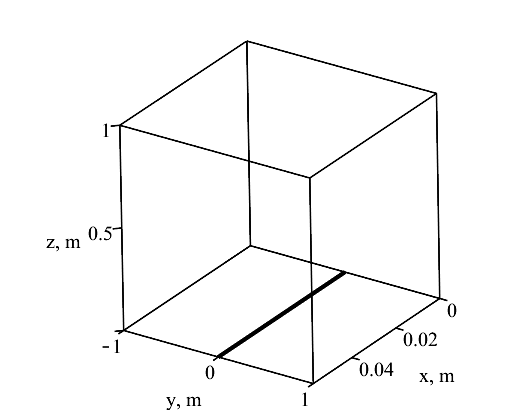
\includegraphics[width=0.95\linewidth]{ModelTrBPR1_.png} \\ а)}
\end{minipage}
\hfill
\begin{minipage}[t]{0.3\linewidth}
	\center{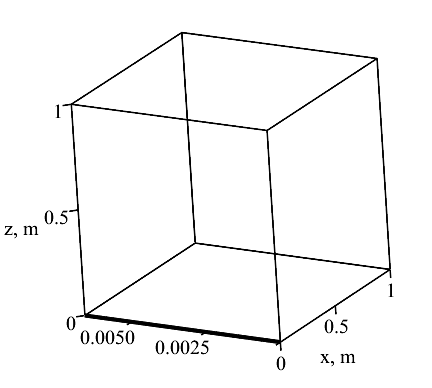
\includegraphics[width=0.95\linewidth]{ModelTrBPR2_.png} \\ б)}
\end{minipage}
\hfill
\begin{minipage}[t]{0.3\linewidth}
	\center{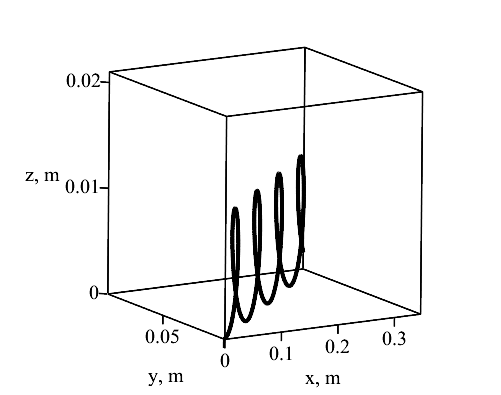
\includegraphics[width=1\linewidth]{ModelTrBPR12_.png} \\ в)}
\end{minipage}


\end{frame}

\begin{frame}
\frametitle{Экспериментальные исследования}
1.	Вращение пары больших роторов. $K = (2i_1\omega_{max}, 0, 0)$.


	\begin{minipage}[t]{0.3\linewidth}
		\center{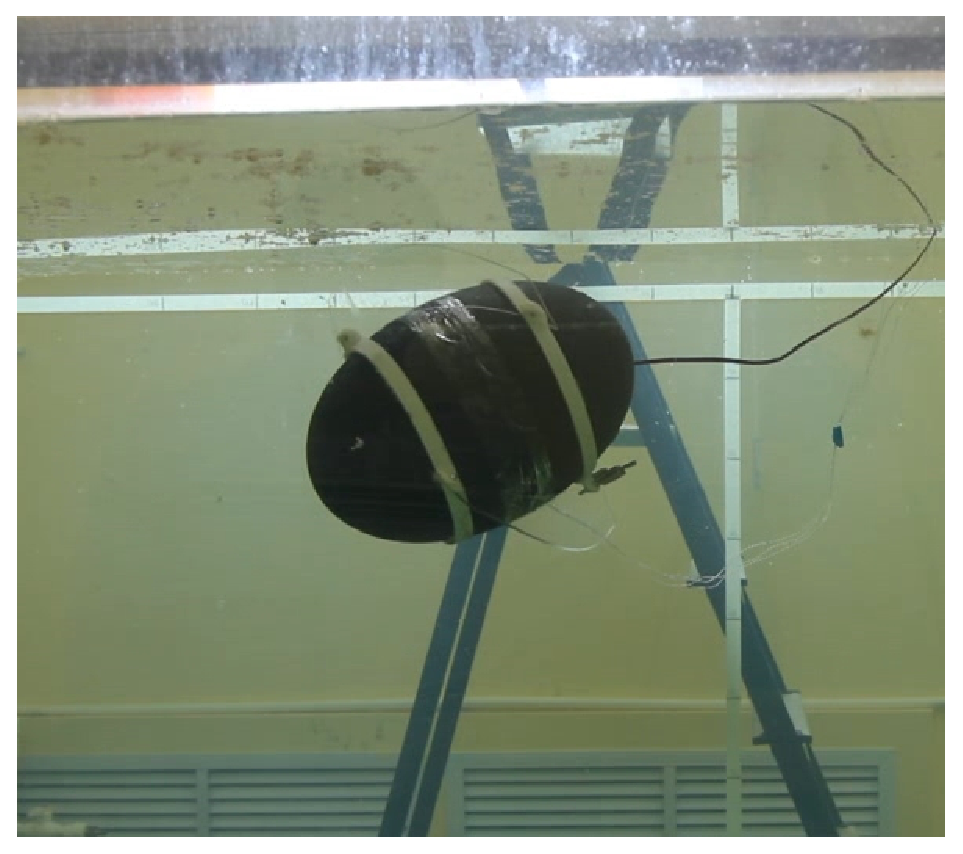
\includegraphics[width=0.7\linewidth]{exp11.eps} \\ а)}
	\end{minipage}
	\hfill
	\begin{minipage}[t]{0.3\linewidth}
		\center{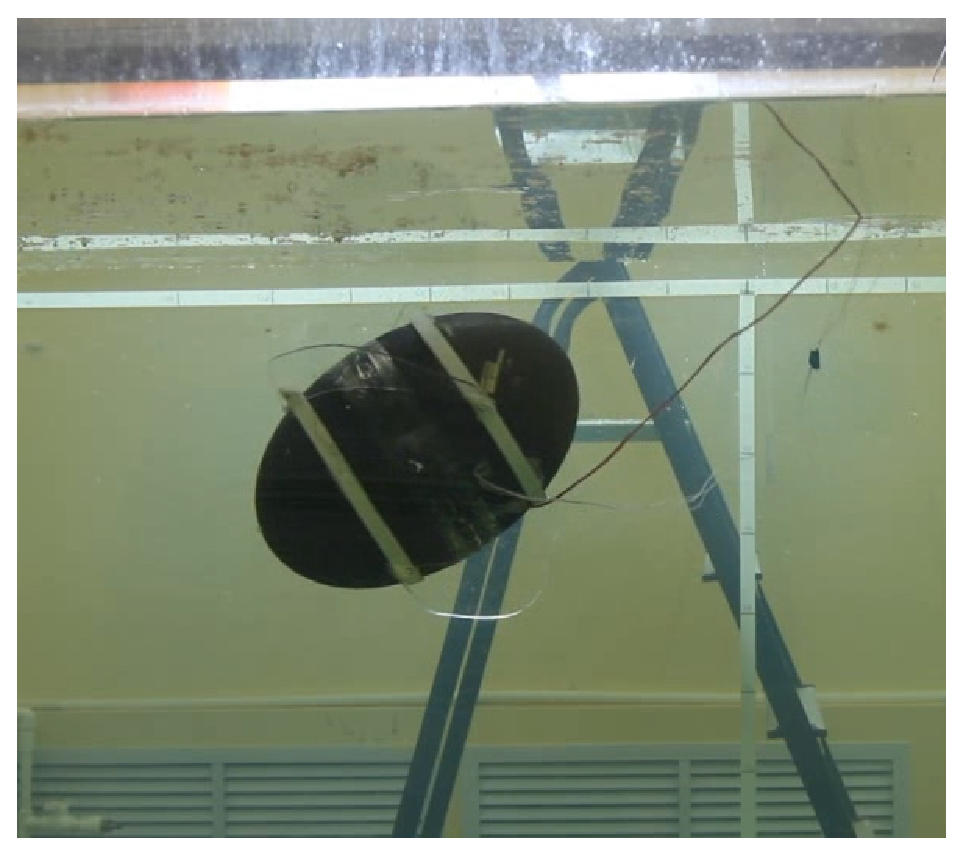
\includegraphics[width=0.7\linewidth]{exp12.eps} \\ б)}
	\end{minipage}
	\hfill
	\begin{minipage}[t]{0.3\linewidth}
		\center{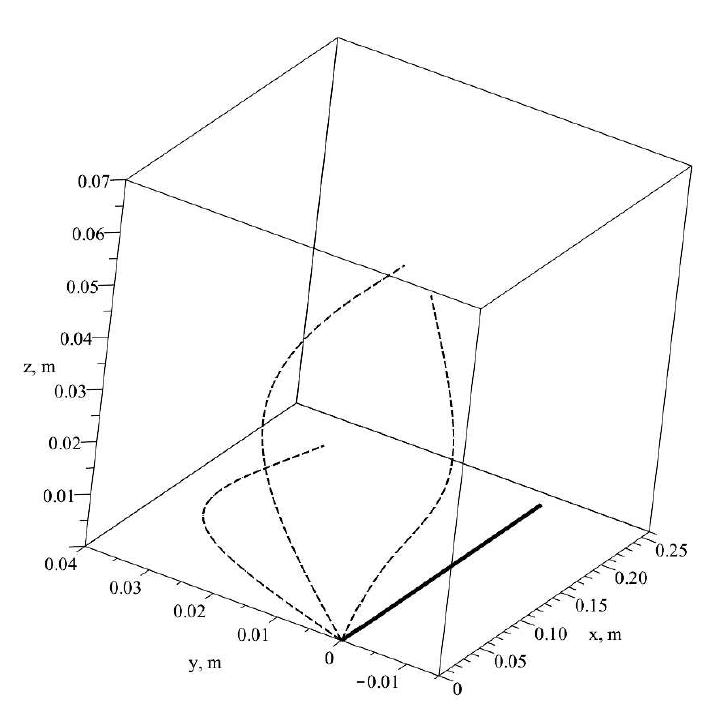
\includegraphics[width=0.8\linewidth]{Exp_BPR_1.png} \\ в)}
	\end{minipage}


Положение робота а) в начальный момент времени и б) момент времени t=3 секунды от начала движения; в) теоретическая (сплошная линия) и экспериментальные (штриховые линии) траектории движения безвинтового подводного робота 

\begin{table}[h]
	\centering
	\begin{tabular}{|c|c|c|c|c|c|c|c|}
		\hline
		& $\Delta x$, м & $\Delta y$, м & $\Delta z$, м & $|\br_t|$, м & $\Delta \theta$ & $\Delta \psi$ & $\Delta \varphi$ \\ \hline
		Теория & $0.275$ & $0$ & $0$ & $0.275$ & $ 0^{\circ}$ & $ 0^{\circ}$ & $ 738.2^{\circ}$ \\ \hline
		Эксперимент & $0.115$  & $0.010$ & $0.055$ & $0.128$ & $ 4^{\circ} $ & $ 10^{\circ} $ & $ 121^{\circ} $  \\
		\hline
	\end{tabular}
\end{table}

\end{frame}


\begin{frame}
\frametitle{Экспериментальные исследования}
2.	Вращение одной пары малых роторов. $K = (0, 2i_2\omega_{max}, 0)$. 


	\begin{minipage}[h]{0.3\linewidth}
		\center{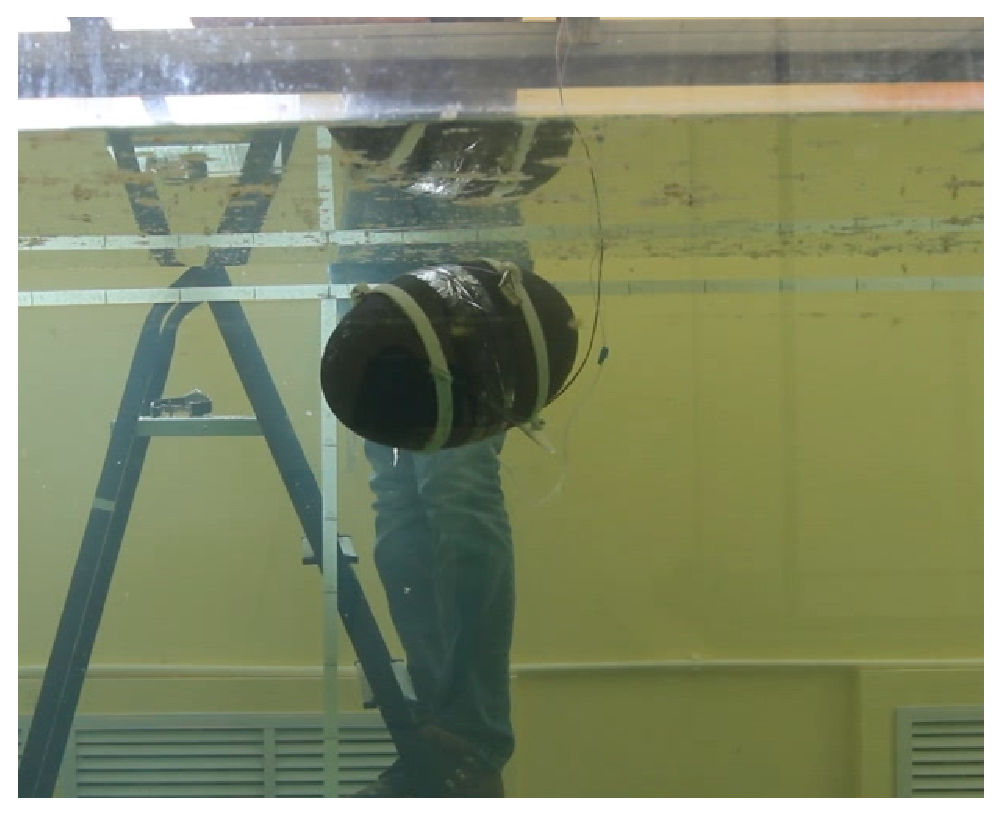
\includegraphics[width=0.7\linewidth]{exp21.eps} \\ а)}
	\end{minipage}
	\hfill
	\begin{minipage}[h]{0.3\linewidth}
		\center{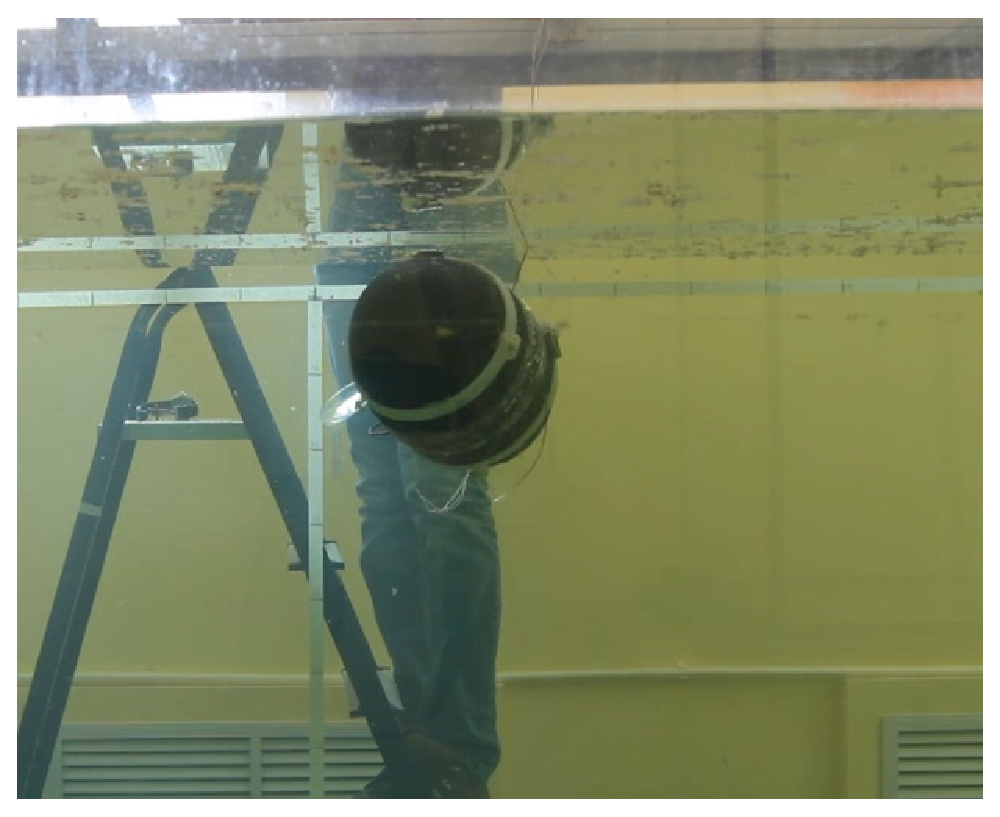
\includegraphics[width=0.7\linewidth]{exp22.eps} \\ б)}
	\end{minipage}
	\hfill
	\begin{minipage}[h]{0.3\linewidth}
		\center{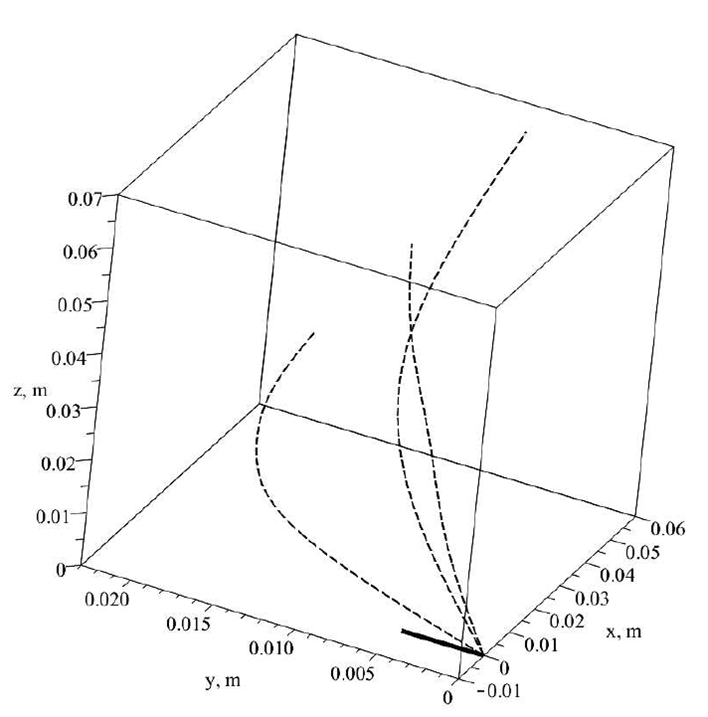
\includegraphics[width=0.8\linewidth]{Exp_BPR_2.png} \\ в)}
	\end{minipage}


Положение робота а) в начальный момент времени и б) момент времени t=3 секунды от начала движения; в) теоретическая (сплошная линия) и экспериментальные (штриховые линии) траектории движения безвинтового подводного робота 

\begin{table}[h]
	\centering
	\begin{tabular}{|c|c|c|c|c|c|c|c|}
		\hline
		& $\Delta x$, м & $\Delta y$, м & $\Delta z$, м & $|\br_t|$, м & $\Delta \theta$ & $\Delta \psi$ & $\Delta \varphi$ \\ \hline
		Теория & $0$ & $0.005$ & $0$ & $0.005$ & $ 35^{\circ}$ & $ 0^{\circ}$ & $ 0^{\circ}$ \\ \hline
		Эксперимент & $0.054$  & $0.008$ & $0.068$ & $0.087$ & $ 61^{\circ} $ & $ 62^{\circ} $ & $ 10^{\circ} $  \\
		\hline
	\end{tabular}
\end{table}

\end{frame}


\begin{frame}
\frametitle{Экспериментальные исследования}
3.	Вращение пары больших роторов и одной пары малых роторов. $K = (2i_1\omega_{max}, 2i_2\omega_{max}, 0)$. 

	\begin{minipage}[h]{0.3\linewidth}
		\center{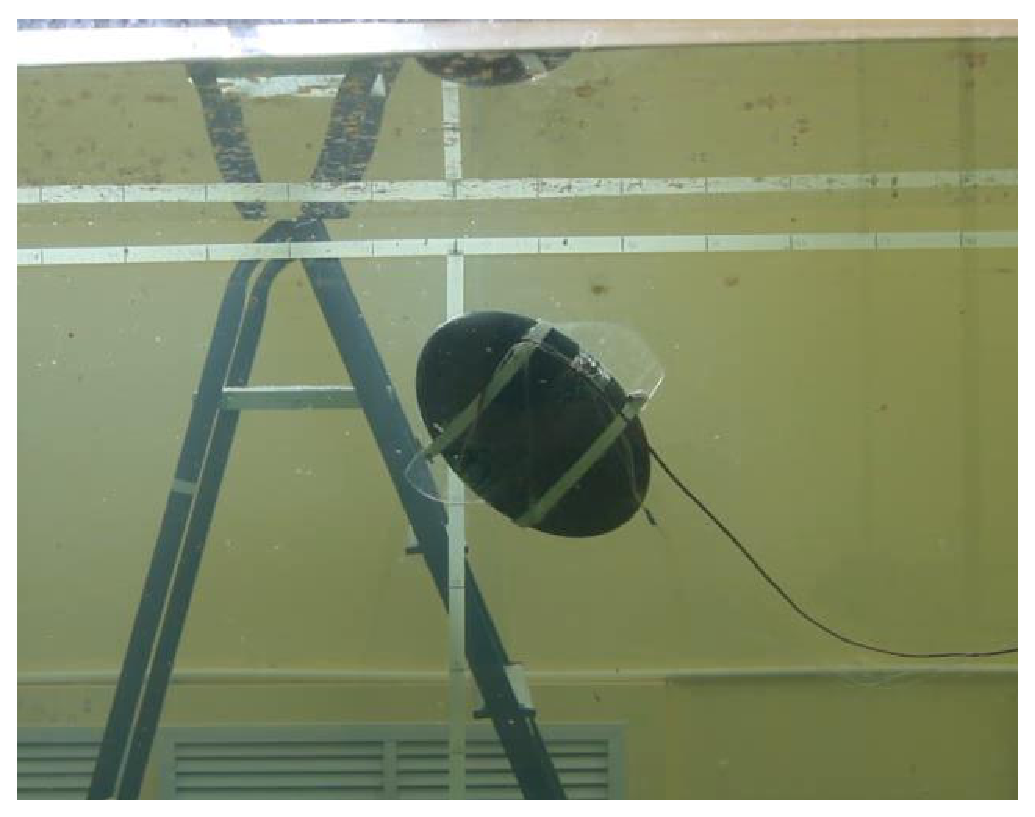
\includegraphics[width=0.7\linewidth]{exp31.eps} \\ а)}
	\end{minipage}
	\hfill
	\begin{minipage}[h]{0.3\linewidth}
		\center{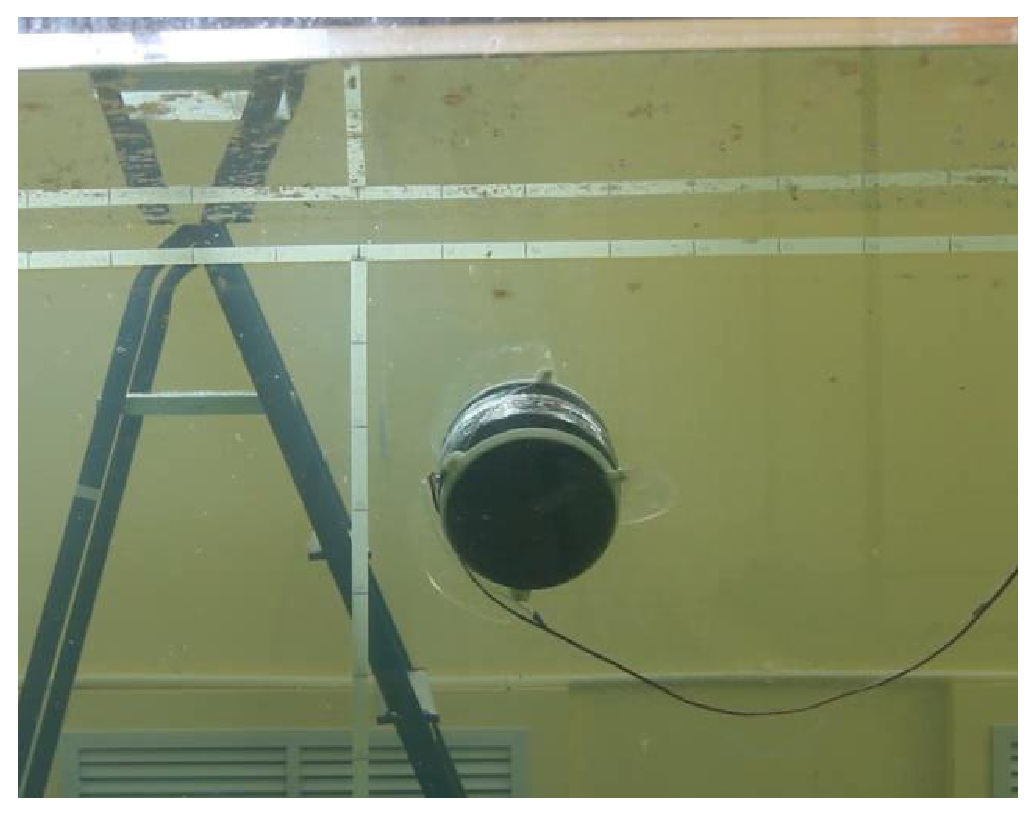
\includegraphics[width=0.7\linewidth]{exp32.eps} \\ б)}
	\end{minipage}
	\hfill
	\begin{minipage}[h]{0.3\linewidth}
		\center{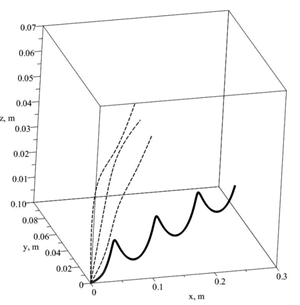
\includegraphics[width=0.8\linewidth]{Exp_BPR_3.png} \\ в)}
	\end{minipage}

Положение робота а) в начальный момент времени и б) момент времени t=3 секунды от начала движения; в) теоретическая (сплошная линия) и экспериментальные (штриховые линии) траектории движения безвинтового подводного робота 

\begin{table}[h]
	\centering
	\begin{tabular}{|c|c|c|c|c|c|c|c|}
		\hline
		& $\Delta x$, м & $\Delta y$, м & $\Delta z$, м & $|\br_t|$, м & $\Delta \theta$ & $\Delta \psi$ & $\Delta \varphi$ \\ \hline
		Теория & $0.275$ & $0$ & $0$ & $0.275$ & $ 35^{\circ}$ & $ 0^{\circ}$ & $ 738.2^{\circ}$ \\ \hline
		Эксперимент & $0.106$  & $0.050$ & $0.053$ & $0.189$ & $ 17^{\circ} $ & $ 92^{\circ} $ & $ 51^{\circ} $  \\
		\hline
	\end{tabular}
\end{table}

%\begin{center}
%	$\Delta x_{exp}=0.106\; \mbox{м}, \; \Delta y_{exp}=0.050\; \mbox{м},\; \Delta z_{exp}=0.053\; \mbox{м}, \;$ \\
%	%\item $|r|=0.129$ м;
%	$\Delta \theta_{exp}=17^{\circ},\; \Delta \psi_{exp}=90^{\circ},\; \Delta \varphi_{exp}=51^{\circ}.$
%\end{center}

\end{frame}

\begin{frame}
\frametitle{Закон изменения угловой скорости ротора}

	В общем случае, зависимость угловой скорости ротора от времени будет иметь характерные переходные интервалы, соответствующие разгону и торможению 
	
		\scriptsize 
		\vspace{-4mm}
		\begin{equation*}
		\omega_r(t) =
		\begin{cases}
		
		\omega_1 & t \in \left[ nT;  nT + t_1 \right] ,\\
		
		\frac{(\omega_2 - \omega_1)(t-nT)}{t_2} - \frac{(\omega_2 - \omega_1)(t_1+t_2)}{t_2} + \omega_2 & t \in \left[ nT + t_1;  nT + t_1+t_2 \right], \\
		
		\omega_2 & t \in \left[ nT + t_1+t_2;  nT + t_1+t_2+t_3 \right] ,\\
		
		\frac{(\omega_1 - \omega_2)(t-nT)}{t_4} - \frac{(\omega_1 - \omega_2)(t_1+t_2+t_3+t_4)}{t_4} + \omega_1 &t \in \left[ nT + t_1 + t_2+t_3;  nT + t_1+t_2+t_3+t_4 \right] ,
		
		\end{cases}
		\label{omegaRotorGeneral}
		\end{equation*}
		
		\small
		где $n \in \mathbf{N}$, $T$ -- период управляющего воздействия; $ \omega_1, \omega_2 $ -- амплитуды угловой скорости вращения ротора по часовой стрелке и против часовой стрелки соответственно; $t_1, t_2, t_3, t_4$ -- задают продолжительность по времени характерных интервалов угловой скорости вращения ротора. 
		
			%\framebreak
		
		%Графически данная зависимость приведена на рисунке
		
		\begin{minipage}[t]{0.47\linewidth}
			\begin{figure}[!ht]
				\centering
				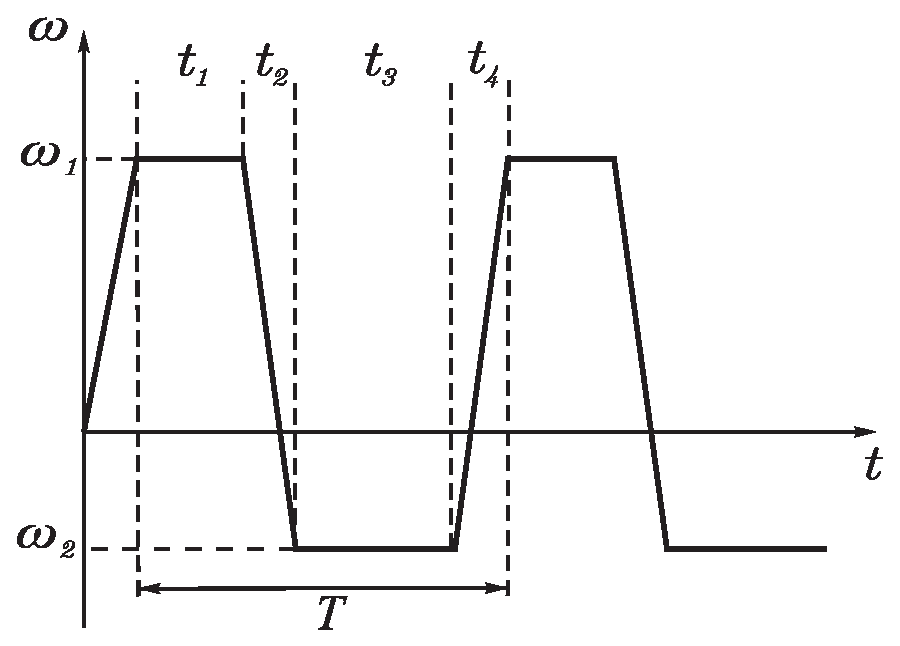
\includegraphics[height=33mm]{ControlAction.eps}
			\end{figure}
			
		\end{minipage}	
		\hfill
		\begin{minipage}[t]{0.47\linewidth}
			\begin{figure}[!ht]
				\centering
				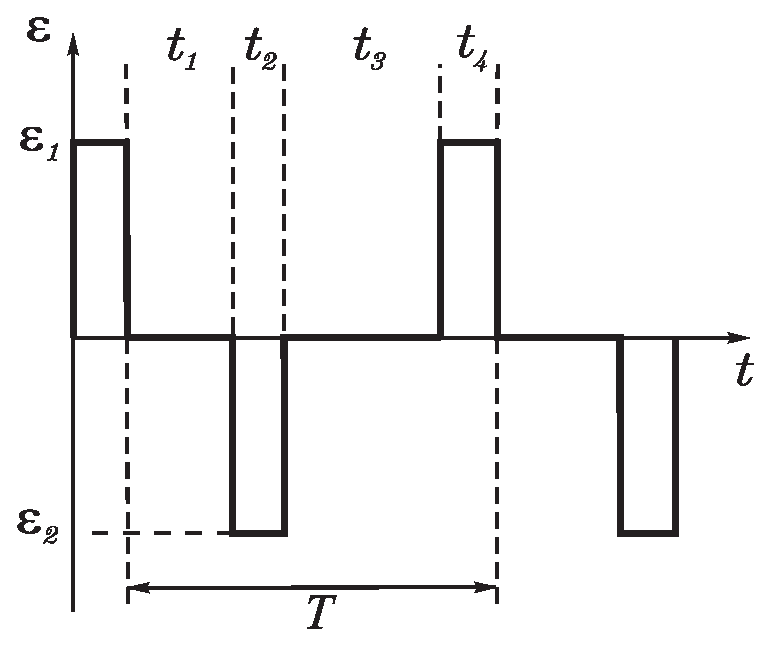
\includegraphics[height=33mm]{ControlActionEpsilon.eps}
			\end{figure}
		\end{minipage}	
%		\begin{figure}[!ht]
%			\centering
%			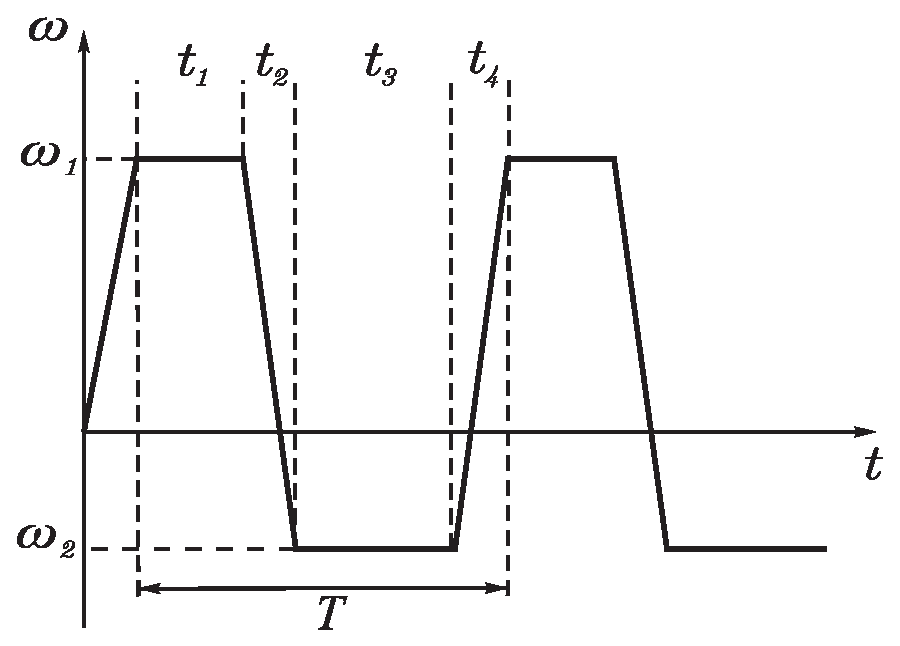
\includegraphics[width=0.4\linewidth]{ControlAction.eps}
%		\end{figure}
	
	
\end{frame}

\begin{frame}
\frametitle{Методика определения коэффициентов}

Уравнения Навье-Стокса, записанные относительно криволинейной системы координат $(\xi,\, \eta)$, связанной с движущимся профилем имеют вид:
\begin{gather*}
\begin{gathered}
\pder{Du_1}{\xi} + \pder{Du_2}{\eta} = 0,\\
\begin{split}
\pder{u_1}{t} + \frac{1}{D^2} \biggl( \pder{D(u_1 - w_1)u_1}{\xi} + & \pder{D(u_2 - w_2)u_1}{\eta} \biggr) = \\
= - \frac{1}{D\rho} \pder{p}{\xi} + & \frac{\nu}{D^2} \left( \pdder{u_1}{\xi}{2} + \pdder{u_1}{\eta}{2} \right) + \beta_1 + 2 u_2 \omega
\end{split}\\
\begin{split}
\pder{u_2}{t} + \frac{1}{D^2} \biggl( \pder{D(u_1 - w_1)u_2}{\xi} + & \pder{D(u_2 - w_2)u_2}{\eta} \biggr) = \\
= - \frac{1}{D\rho} \pder{p}{\eta} + & \frac{1}{D^2} \left( \pdder{u_2}{\xi}{2} + \pdder{u_2}{\eta}{2} \right) + \beta_2 - 2 u_1 \omega,
\end{split}
\end{gathered}
\end{gather*}
где $u_1$, $u_2$ --- проекции вектора скорости жидкости на криволинейные оси, $p$ --- давление, $\rho$ --- плотность жидкости, $\nu$ --- кинематическая вязкость, $w_1 = v_1 - \omega x_2(\xi,\, \eta)$, $w_2 = v_2 + \omega x_1(\xi,\, \eta)$ --- компоненты переносной скорости. 

\end{frame}

\begin{frame}
\frametitle{Методика определения коэффициентов}


Коэффициент Ламэ $D$ и члены $\beta_1$, $\beta_2$, возникающие вследствие искривления сеточных линий, имеют вид:
\begin{gather*}
D = \sqrt{\left( \pder{x_1}{\xi}\right)^2 + \left( \pder{x_2}{\xi}\right)^2  } =\sqrt{\left( \pder{x_1}{\eta}\right)^2 + \left( \pder{x_2}{\eta}\right)^2  },\\
\begin{split}
\beta_1 = \frac{\nu}{D^3} \Biggl( u_1\left( \pdder{D}{\xi}{2} + \pdder{D}{\eta}{2} \right) + {} & {} 2 \pder{u_1}{\xi} \pder{D}{\xi} + 2 \pder{u_2}{\xi} \pder{D}{\eta} + \\
+ {} & {} \frac{2u_2}{D} \pder{D}{\xi} \pder{D}{\eta} - \frac{2u_1}{D} \left( \pder{D}{\eta} \right)^2  \Biggr)
\end{split}\\
\begin{split}
\beta_2 = \frac{\nu}{D^3} \Biggl( u_2\left( \pdder{D}{\xi}{2} + \pdder{D}{\eta}{2} \right) + {} & {} 2 \pder{u_1}{\eta} \pder{D}{\xi} + 2 \pder{u_2}{\eta} \pder{D}{\eta} + \\
+ {} & {} \frac{2u_1}{D} \pder{D}{\xi} \pder{D}{\eta} - \frac{2u_2}{D} \left( \pder{D}{\xi}\right)^2 \Biggr)
\end{split}
\end{gather*}

\end{frame}




\begin{frame}
\frametitle{Методика определения коэффициентов}

При известных распределениях $u_1$, $u_2$, $p$ cилы $f_1$, $f_2$ и момент $g$, действующие на тело со стороны жидкости, определяются следующими интегралами по контуру $L$ профиля:
\begin{gather*}
\begin{gathered}
f_1 = \oint_L \left( p \pder{x_2}{\xi} + \frac{\rho \nu}{D} \pder{u_1}{\eta} \pder{x_1}{\xi} \right) d\xi,\\
f_2 = \oint_L \left( -p \pder{x_1}{\xi} + \frac{\rho \nu}{D} \pder{u_1}{\eta} \pder{x_2}{\xi} \right) d\xi,\\
g = \oint_L \left( x_1 \left( -p \pder{x_1}{\xi} + \frac{\rho \nu}{D} \pder{u_1}{\eta} \pder{x_2}{\xi} \right) - x_2 \left( p \pder{x_2}{\xi} + \frac{\rho \nu}{D} \pder{u_1}{\eta} \pder{x_1}{\xi} \right) \right) d\xi - \dot{k}(t).
\end{gathered}\label{eq.fgNS}
\end{gather*}

Поскольку движение робота является существенно нестационарным, оказывается невозможным определение коэффициентов $\lambda_{11}$, $\lambda_{22}$, $\lambda_{33}$, $\lambda_{23}$, $c_1$, $c_2$, $c_3$ по-отдельности. Таким образом данные коэффициенты должны определяться совместно с учетом нестационарности движение профиля.

%	Для задания граничных условий, соответствующих нестационарному движению профиля, будем использовать экспериментальные данные для прототипа, описанного в разделе 1 с периодом управляющего воздействия $T = 1$ с, которые представляют собой таблицу значений:
%	\begin{gather}
%	(t_i,\, x_i,\, y_i,\, \alpha_i),\quad i = 0,\, \ldots,\, N.\label{eq.expXYPhi}
%	\end{gather}
%	Здесь $t_i$ --- момент времени, $(x_i,\, y_i)$ --- положение центра масс профиля в момент времени $t_i$, $\alpha_i$ --- ориентация профиля в момент времени $t_i$.
%	
\begin{gather*}
\begin{gathered}
\lambda_{11}^{(1)} \approx 0.3087, \quad 
\lambda_{22}^{(1)} \approx -0.5796,\quad 
\lambda_{23}^{(1)} \approx 0.039085,\\
\lambda_{22}^{(2)} \approx 2.0996,\quad 
\lambda_{23}^{(2)} \approx 0.17629,\quad
\lambda_{11}^{(2)} \approx -7.9826,\\
\lambda_{23,l}^{(3)} \approx 0.083474,\quad
\lambda_{33}^{(2)} \approx 0.018935,\quad
\lambda_{11}^{(3)} - \lambda_{22}^{(3)} \approx - 4.7550,\quad
\lambda_{23,r}^{(3)} \approx 1.4488,\\
c_1 = 0.04715,\quad c_2 = 17.702,\quad c_3 = 0.092872.
\end{gathered}\label{eq.coeffs2}
\end{gather*}


\end{frame}